\documentclass[Space3_Assign2]{subfile}

\begin{document}

\begin{figure}
\centering
\caption{GPS 24 hr simulation with dt = 100 in ECI frame}
\label{Q1AECI}
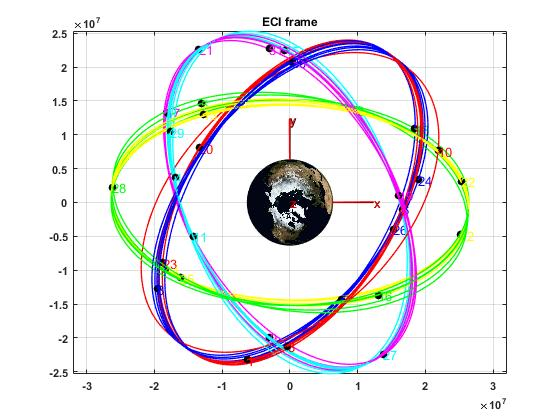
\includegraphics[width = \linewidth]{./Q1AECI.jpg}
\end{figure}

\begin{figure}
\centering
\caption{GPS 24 hr simulation with dt = 100 in ECI frame}
\label{Q1AECIside}
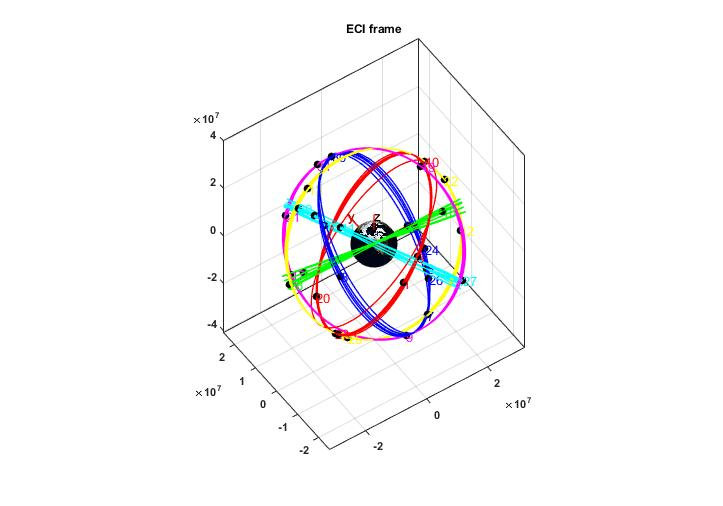
\includegraphics[width = \linewidth]{./Q1AECI_side.jpg}
\end{figure}

\begin{figure}
\centering
\caption{GPS 24 hr simulation with dt = 100 in ECEF frame}
\label{Q1AECEF}
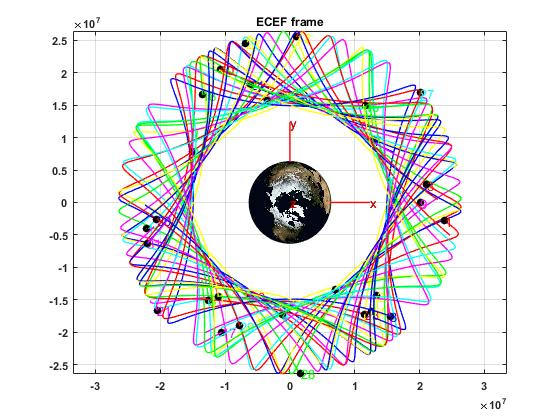
\includegraphics[width = \linewidth]{./Q1AECEF.jpg}
\end{figure}

\begin{figure}
\centering
\caption{GPS 24 hr simulation with dt = 100 in ECEF frame}
\label{Q1AECEFside}
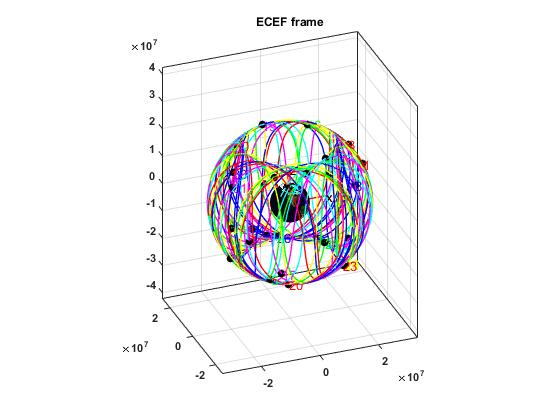
\includegraphics[width = \linewidth]{./Q1AECEF_side.jpg}
\end{figure}

\begin{figure}
\centering
\caption{GPS 24 hr simulation with dt = 100 Ground Trace}
\label{Q1AGT}
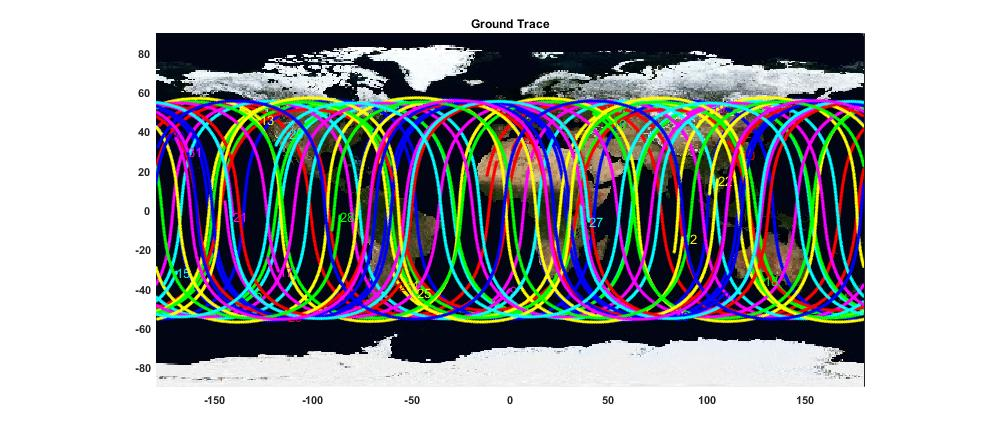
\includegraphics[width = \linewidth]{./Q1AGT.jpg}
\end{figure}

\begin{figure}
\centering
\caption{UAV Flight 1 trace in NED coordinates from the ground station at [Lat 34.76\Deg,Long: 150.03\Deg E, Alt: 680m]}
\label{Q1BF1LG}
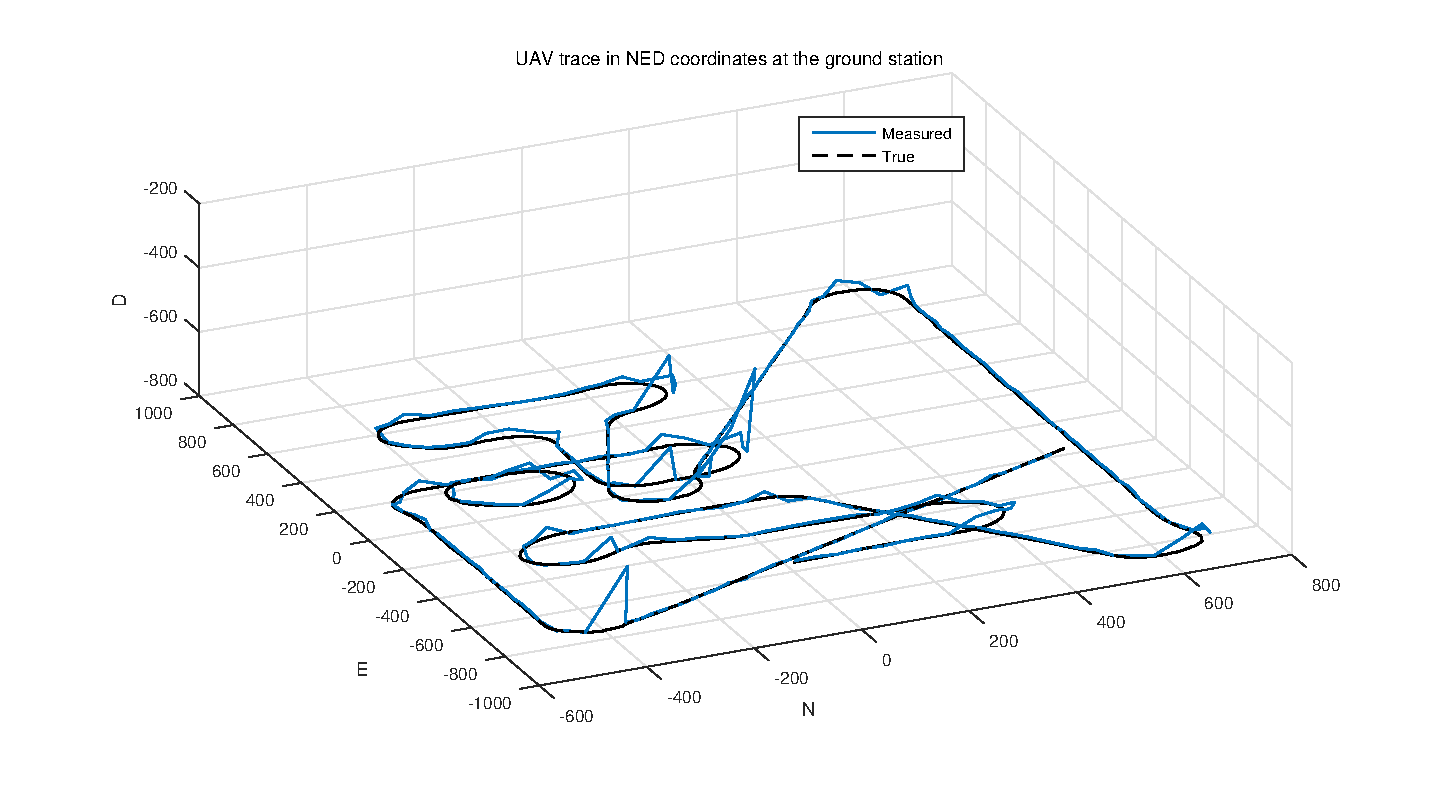
\includegraphics[width = \linewidth]{./Q1B_F1_LG.eps}
\end{figure}

\begin{figure}
\centering
\caption{UAV Flight 1 polar trace of azimuth and elevation and location of observed satellites from ground station at [Lat 34.76\Deg,Long: 150.03\Deg E, Alt: 680m]}
\label{Q1B_polartrack}
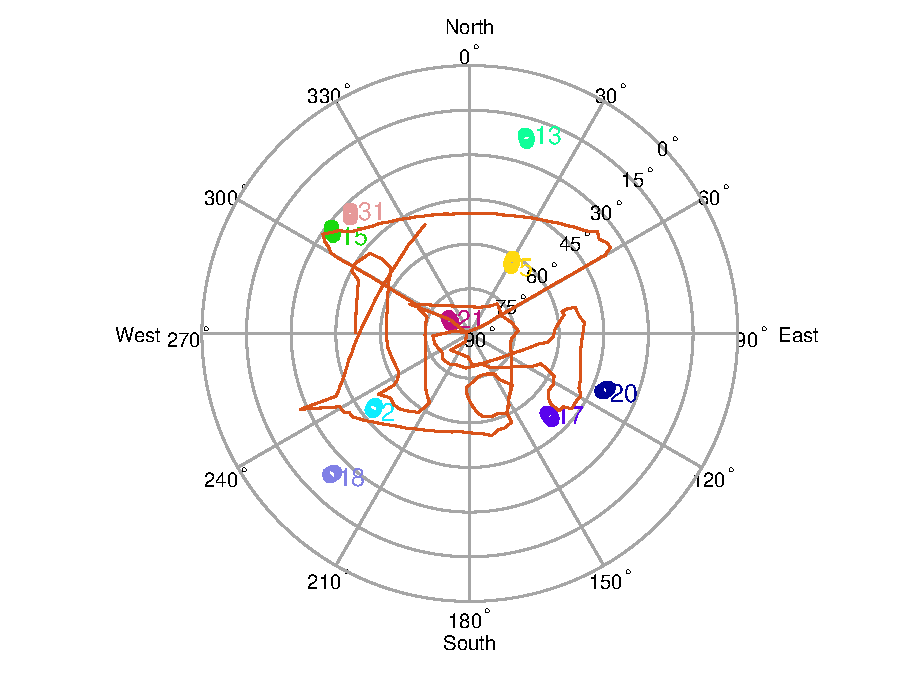
\includegraphics[width = \linewidth]{./Q1B_polartrack.eps}
\end{figure}

\begin{figure}
\centering
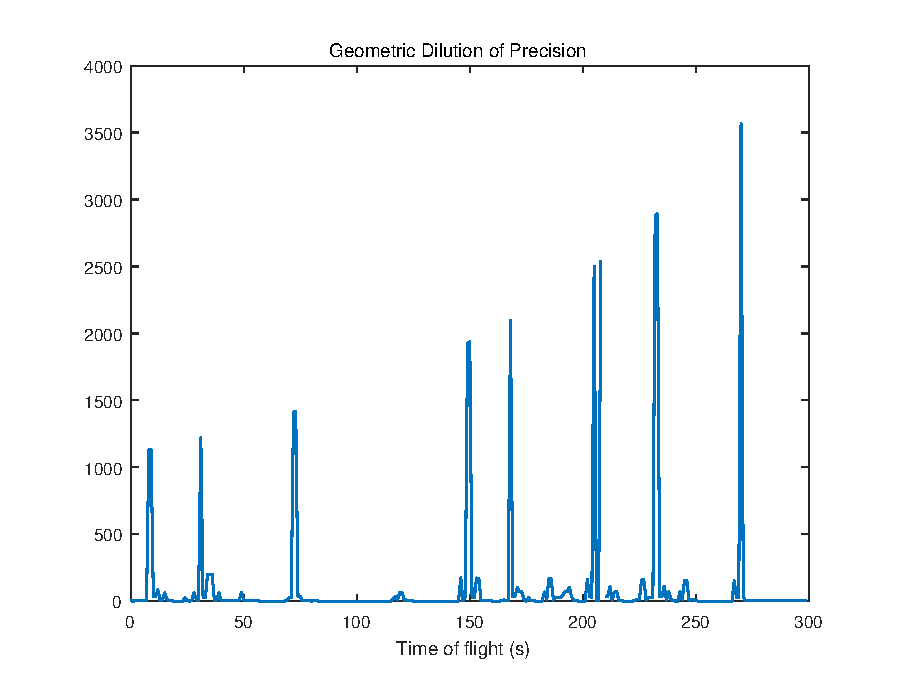
\includegraphics[width=0.8\linewidth]{DOPall.eps}
\caption{Geometric Dilution of Precision for all time of Flight 1}
\label{fig:DOPall}
\end{figure}
\begin{figure}
\centering
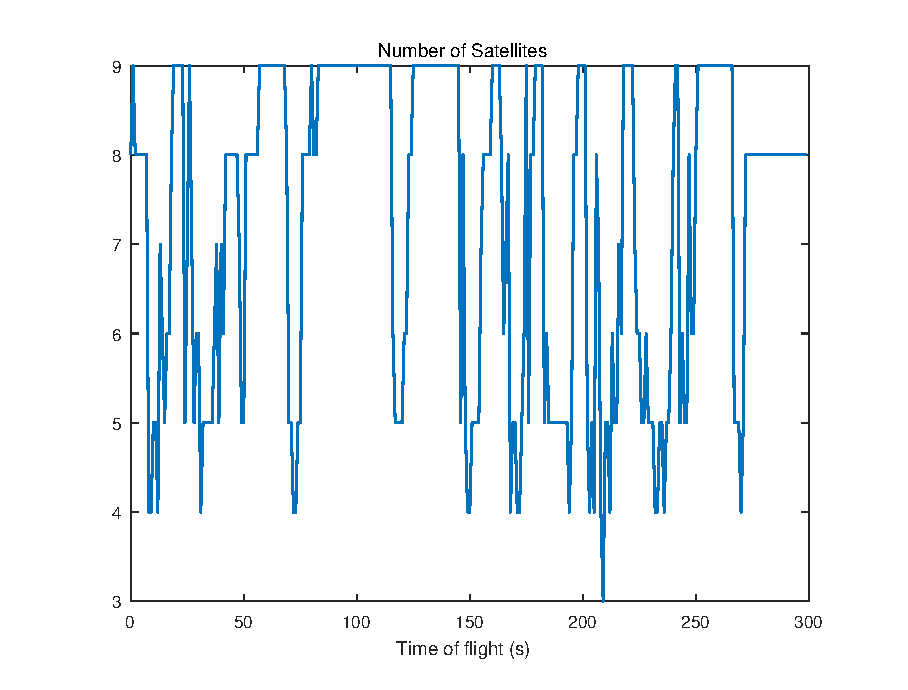
\includegraphics[width=0.8\linewidth]{SatNo.eps}
\caption{Number of Satellites observed of Flight 1}
\label{fig:SatNo}
\end{figure}
\begin{figure}
\centering
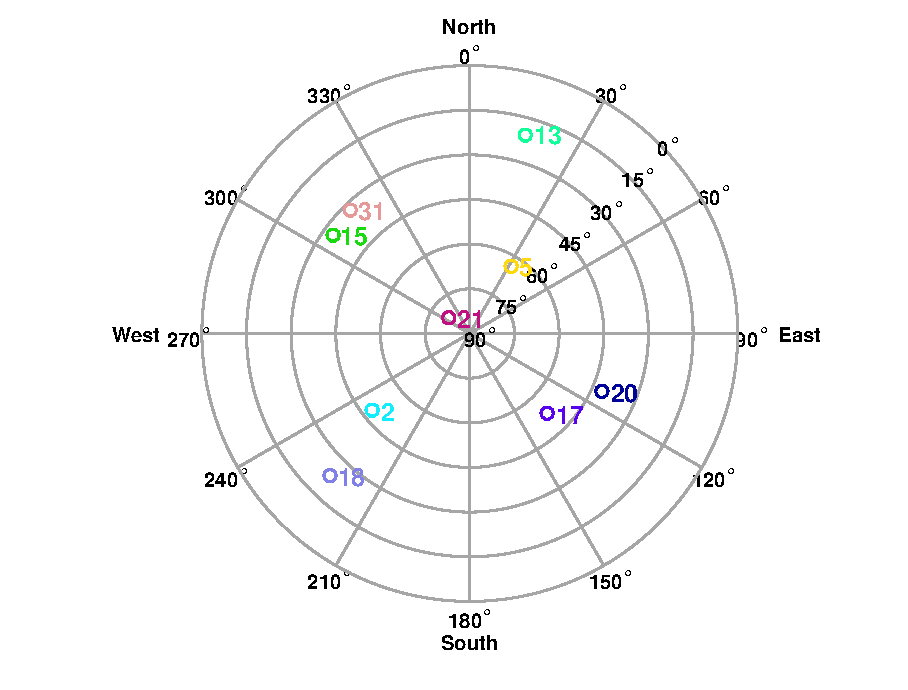
\includegraphics[width=0.8\linewidth]{BestDOP.eps}
\caption{Best GDOP of Flight 1 = 2.747}
\label{fig:BestDOP}
\end{figure}
\begin{figure}
\centering
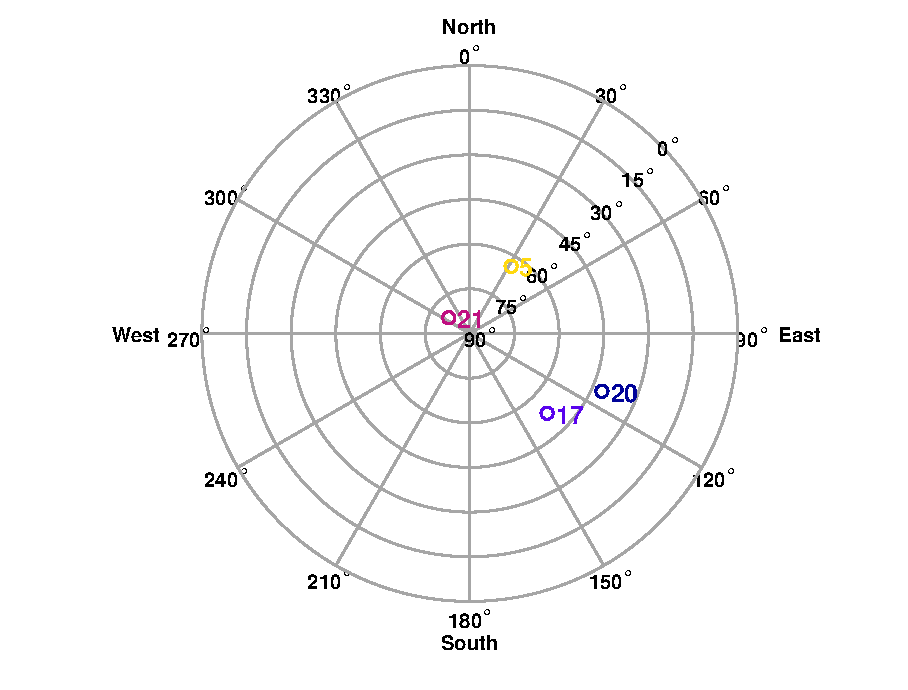
\includegraphics[width=0.8\linewidth]{WorstDOP.eps}
\caption{Worst GOP of Flight 1 = 3567}
\label{fig:WorstDOP}
\end{figure}
\begin{figure}
\centering
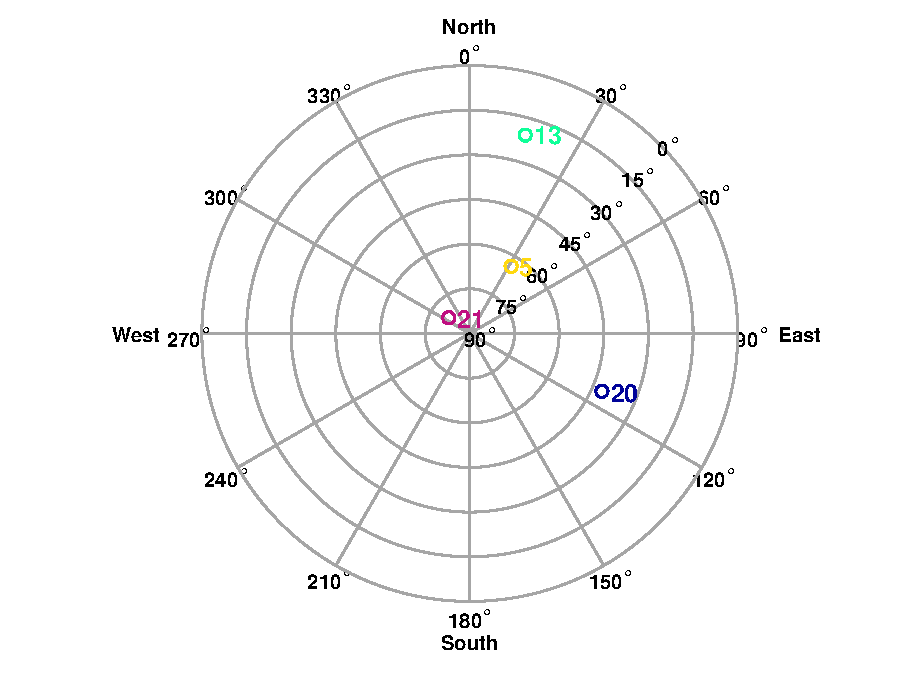
\includegraphics[width=0.8\linewidth]{BestDOP4.eps}
\caption{Best GOP with 4 satellites of Flight 1 = 36.96}
\label{fig:BestDOP4}
\end{figure}

\begin{figure}
\centering
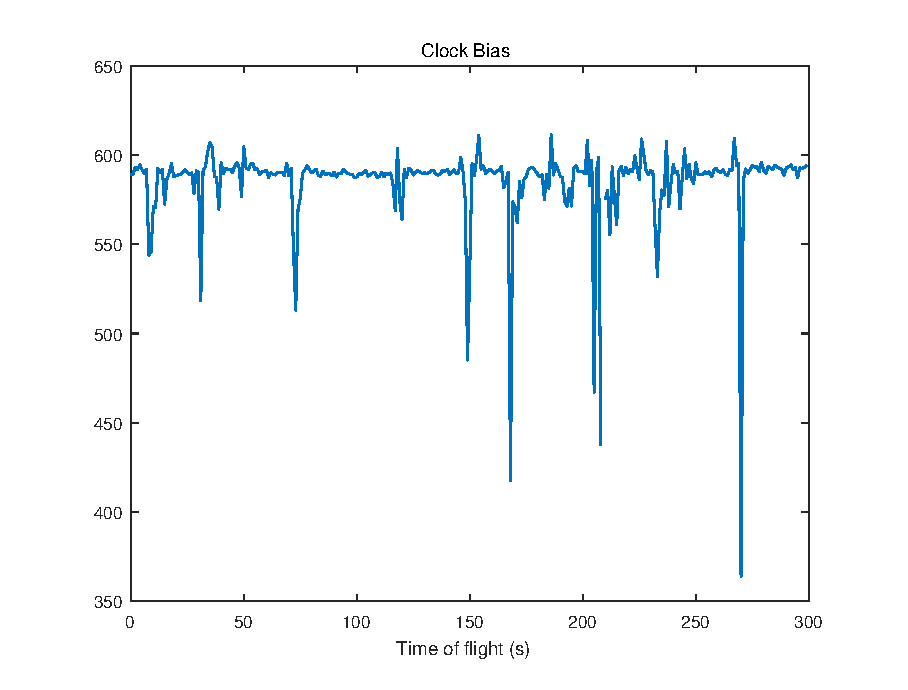
\includegraphics[width=0.8\linewidth]{clockbias}
\caption{Clock Bias of Flight 1}
\label{fig:clockbias}
\end{figure}

\begin{figure}
\centering
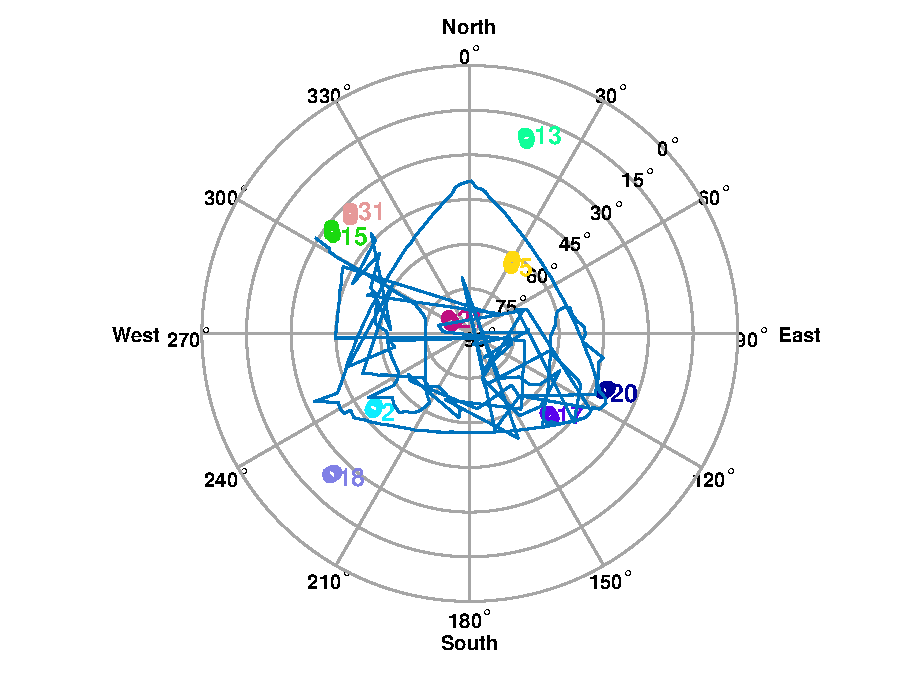
\includegraphics[width=0.8\linewidth]{1Cpolar.eps}
\caption{UAV Flight 2 polar trace of azimuth and elevation and location of observed satellites from ground station at [Lat 34.76\Deg,Long: 150.03\Deg E, Alt: 680m]}
\label{fig:1Cpolar}
\end{figure}
\begin{figure}
\centering
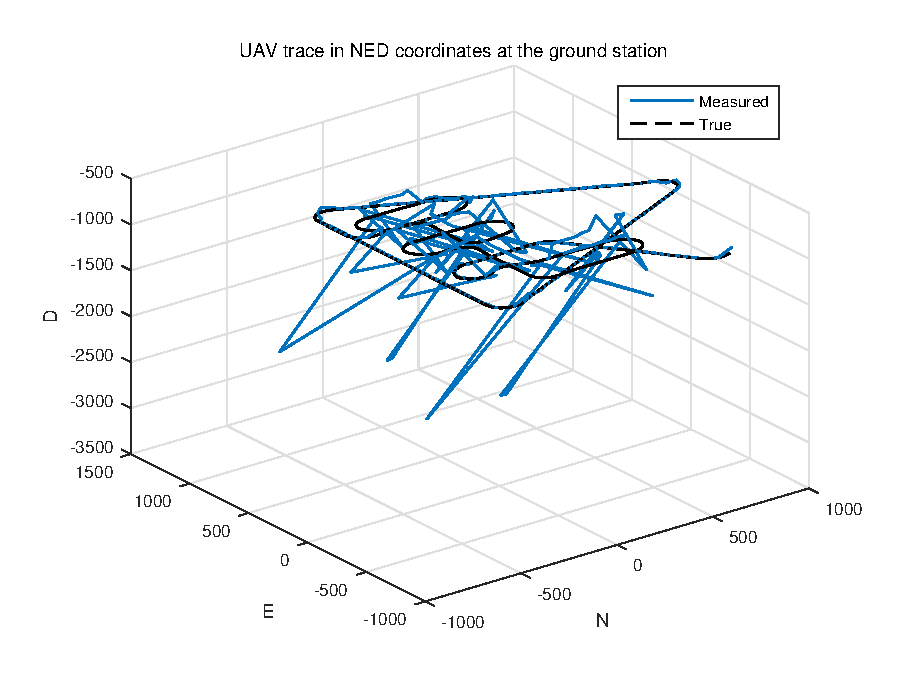
\includegraphics[width=0.8\linewidth]{1Ccart.eps}
\caption{UAV Flight 2 trace in NED coordinates from the ground station at [Lat 34.76\Deg,Long: 150.03\Deg E, Alt: 680m]}
\label{fig:1Ccart}
\end{figure}
\begin{figure}
\centering
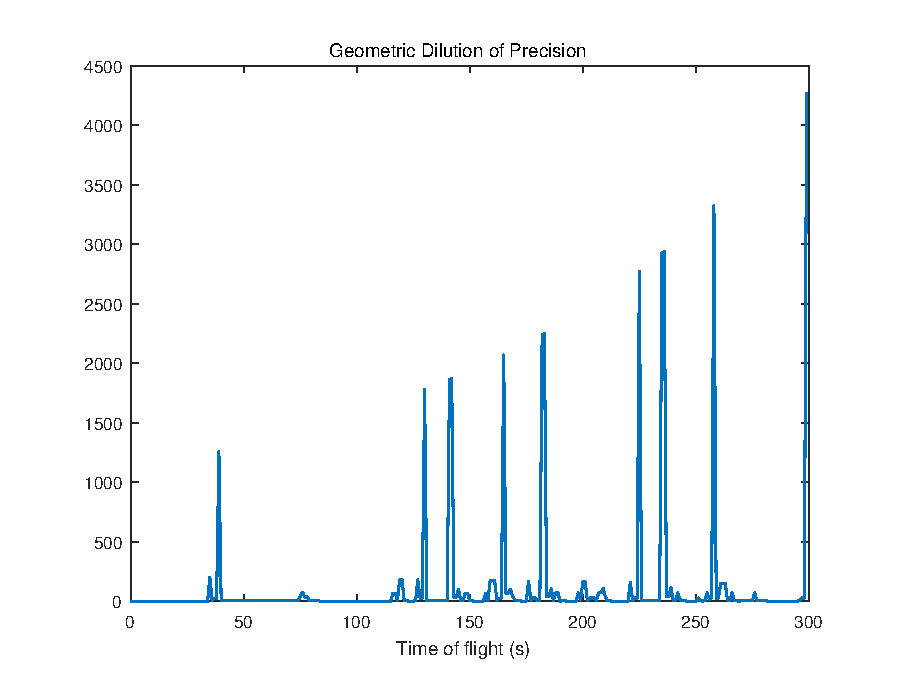
\includegraphics[width=0.8\linewidth]{1Cgopall.eps}
\caption{Geometric DOP for all time Flight 2}
\label{fig:1Cgopall}
\end{figure}
\begin{figure}
\centering
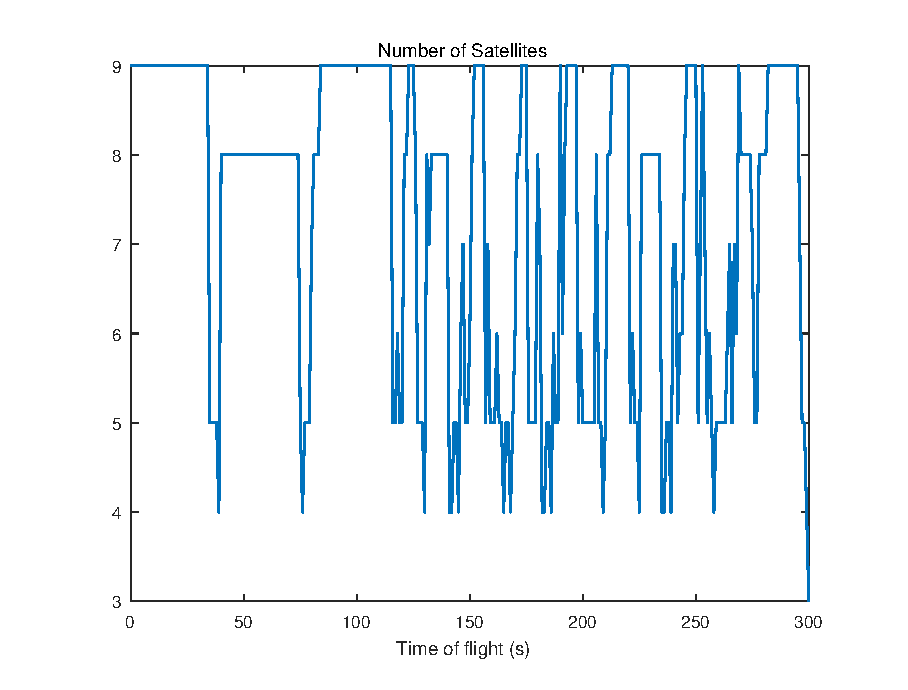
\includegraphics[width=0.8\linewidth]{1cnumsats.eps}
\caption{Number of satellites observed Flight 2}
\label{fig:1cnumsats}
\end{figure}
\begin{figure}
\centering
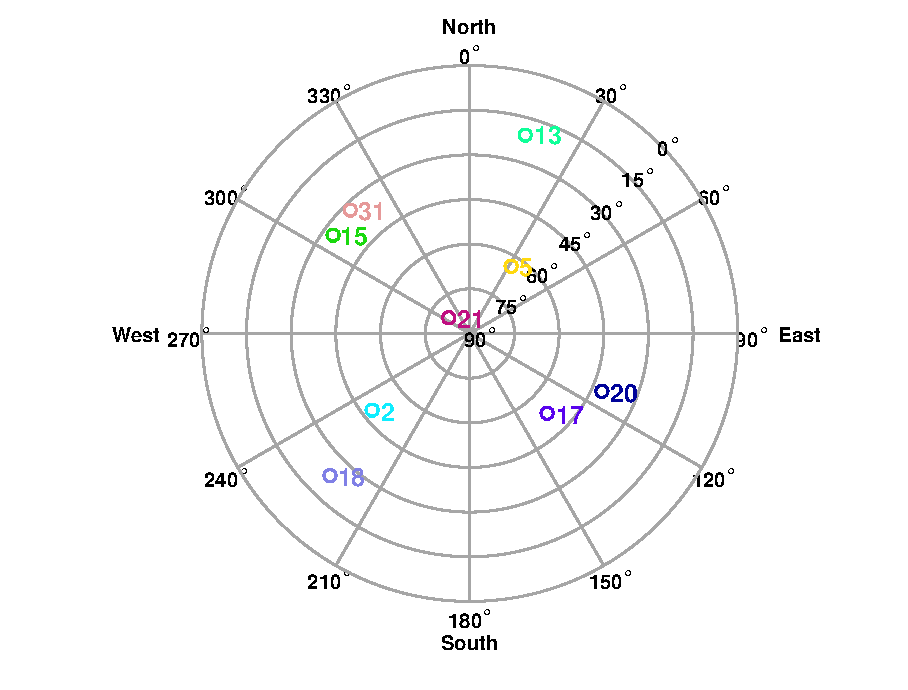
\includegraphics[width=0.7\linewidth]{1Cbest.eps}
\caption{Best GDOP of Flight 2 = 2.74}
\label{fig:1Cbest}
\end{figure}
\begin{figure}
\centering
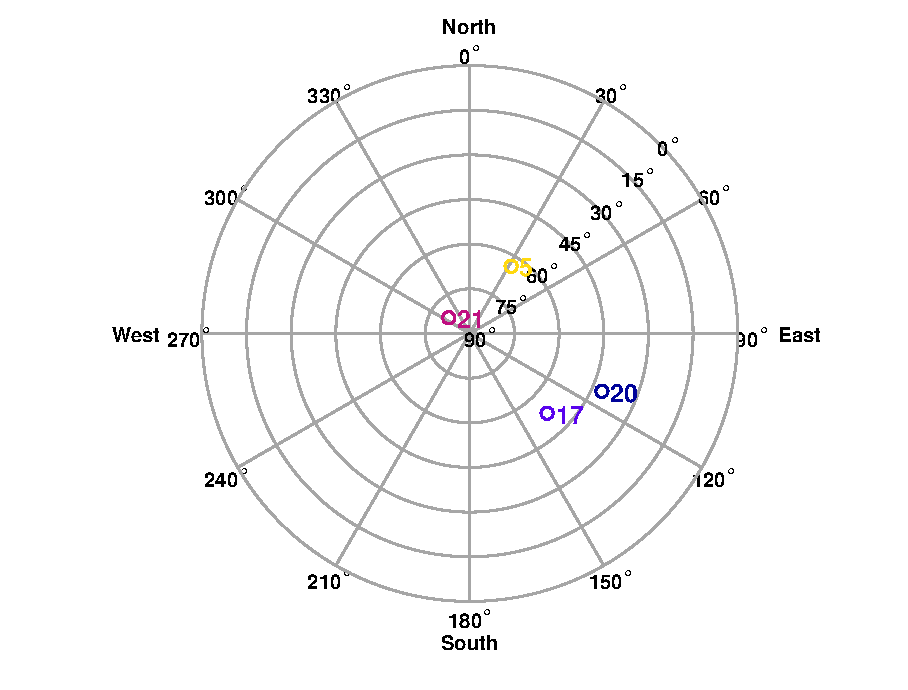
\includegraphics[width=0.7\linewidth]{1Cwrost.eps}
\caption{Worst GDOP of Flight 2 = 4274}
\label{fig:1Cwrost}
\end{figure}
\begin{figure}
\centering
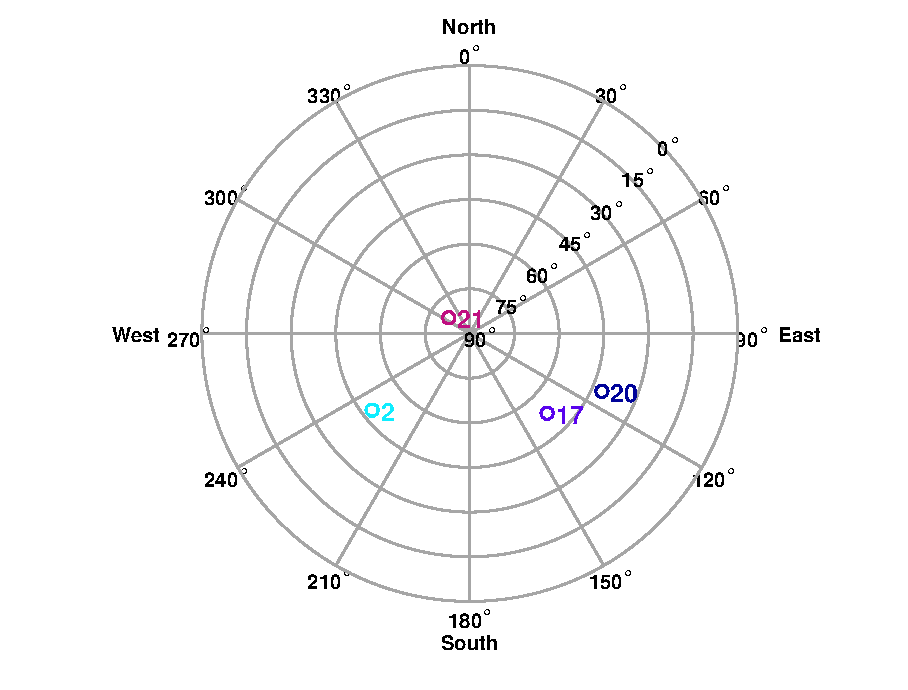
\includegraphics[width=0.7\linewidth]{1Cbest4.eps}
\caption{Best GDOP with four satellites of Flight 2 = 77.5}
\label{fig:1Cbest4}
\end{figure}
\begin{figure}
\centering
\includegraphics[width=0.7\linewidth]{1cerrorandclock.eps}
\caption{Clock Bias of Flight 2 with detection of errors}
\label{fig:1cclockbias}
\end{figure}



\end{document}